\documentclass[conference,compsoc,11pt]{IEEEtran}

\usepackage{multirow}

\usepackage[style=verbose]{biblatex}
\addbibresource{./bibliography.bib}

\ifCLASSINFOpdf
\else
\fi

\usepackage{graphicx}
\graphicspath{ {../misc/} }

\begin{document}
\title{Convolutional Neural Network:\\ Plants Species Classification
\\ \large Artificial Neural Networks and Deep Learning -- A.Y. 2022/2023}

\author{\IEEEauthorblockN{Paolo Botta\IEEEauthorrefmark{1},
Teo Bucci\IEEEauthorrefmark{2} and Silvia Caresana\IEEEauthorrefmark{3}}
\IEEEauthorblockA{M.Sc. Mathematical Engineering,
Politecnico di Milano - Milan, Italy\\
Email: \IEEEauthorrefmark{1}paolo.botta@mail.polimi.it,
\IEEEauthorrefmark{2}teo.bucci@mail.polimi.it,
\IEEEauthorrefmark{3}silvia.caresana@mail.polimi.it\\
Student ID: \IEEEauthorrefmark{1}10612869,
\IEEEauthorrefmark{2}10621873,
\IEEEauthorrefmark{3}10630163\\
Codalab Group: ``Just3Neurons''}
}
\maketitle

%\begin{abstract}
%\end{abstract}

\IEEEpeerreviewmaketitle

\section{Introduction}
The given dataset consists of 3542 images belonging to 8 different classes. To build the classifier, many choices about the model had to be made. Since the settings that can be tweaked in the model would generate many more configurations than our computational power could handle, we followed an incremental approach. Specifically, we started with a baseline and slowly made choices from there, seeing whether the performance improved or not, trying to understand why and if the outcome was expected.

The task suggests to use Categorical Cross-Entropy as loss function, and as metric we used Accuracy as requested. In addition, we also considered the F1--score per class to better understand the weaknesses of the model.

The dataset was split according to an 85:15 train-validation ratio and the results of this report are the ones we obtained on the validation set.

\section{Data Pipeline}

\subsection{Data Augmentation}

Since the dataset is not very numerous, Data Augmentation was used almost from the beginning in all models, allowing the network to better generalize and have a better performance.

We used \textbf{traditional transformations}: Rotating, Zooming, Flipping, Brightness, Shifting, Shear.
Initially only the first three were used, but adding all of them improved slightly the performance.

We thought of using also more \textbf{advanced transformations} like CutMix or CutOut, but given that the dataset is made of plants more or less homogeneous in each sample, we discarded those options and focused our attention more on the architecture for the time being.

\begin{figure}[h!]
\centering
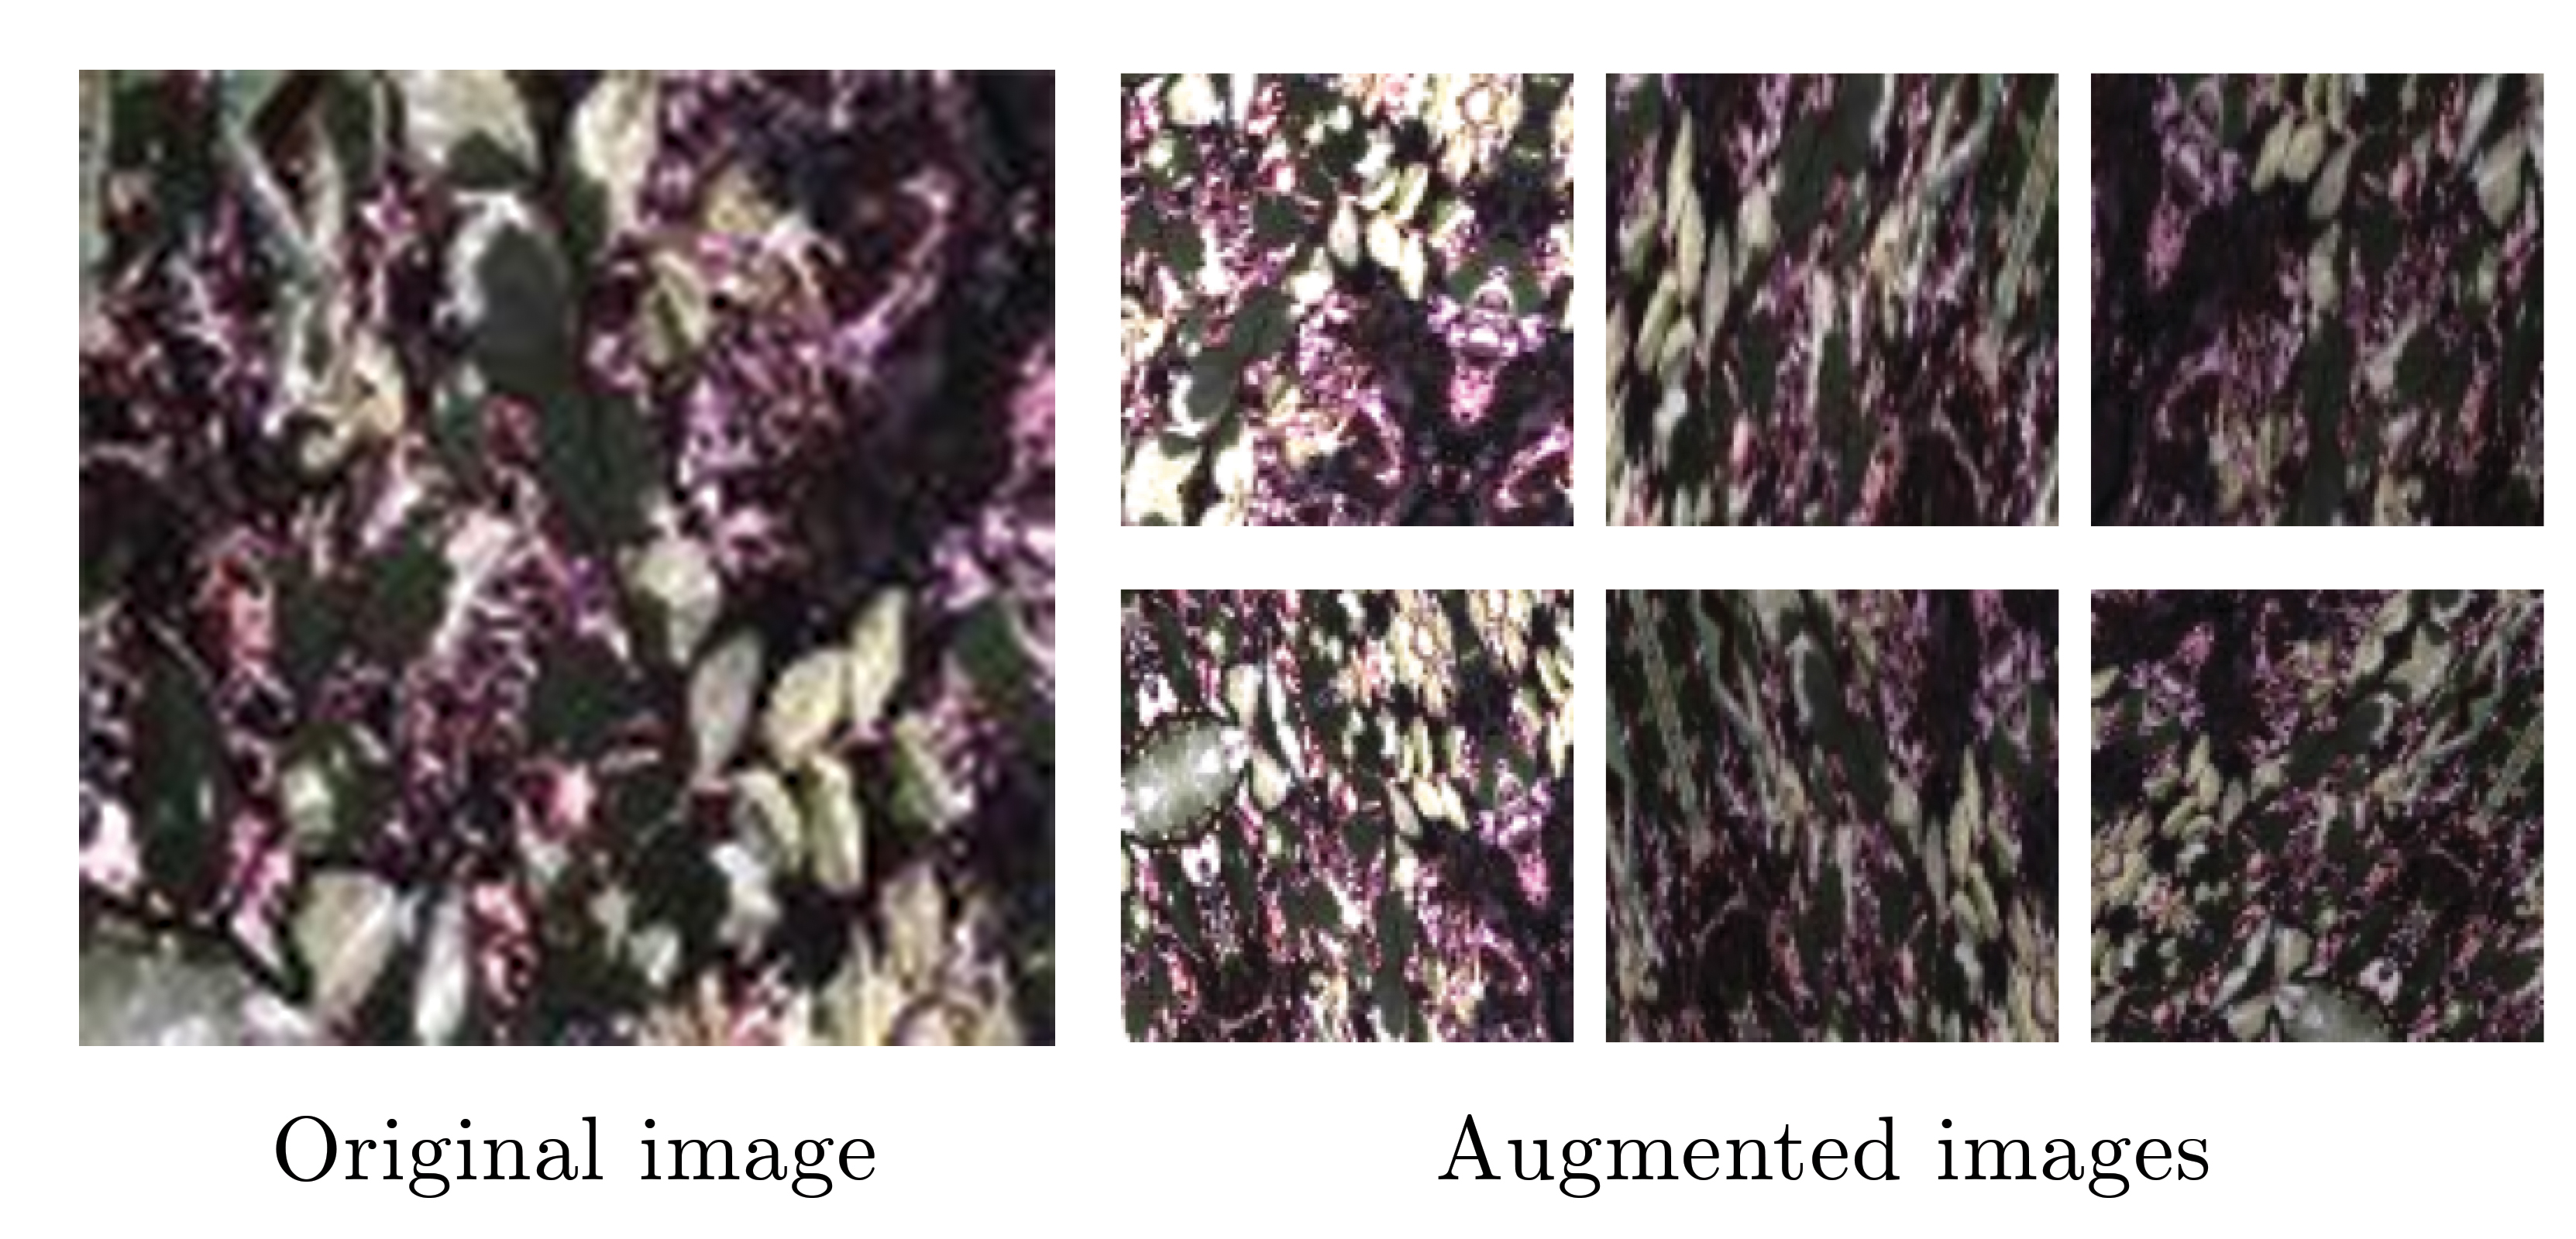
\includegraphics[width=3.1in]{single_augmentation.jpg}
\caption{Some examples of augmented images.}
\end{figure}

\subsection{Test-Time Augmentation}\label{sec:tta}

Once we had our final model (section \ref{sec:model-choice}) we also implemented \textbf{Test-Time Augmentation (TTA)} to build more robust predictions and reduce variance. This gave an improvement of 1.52\% in accuracy.

\subsection{Pre-Processing}

According to the documentation, the Features Extractors (section \ref{sec:features-extractor}) that we chose work best with standardized inputs. Therefore, data processing was done according to the \verb|preprocess_input| contained in \verb|tensorflow.keras.applications|.

\section{Convolutional Neural Network}

We started with a baseline model adopting the classical architecture of modern CNNs. We used 5 blocks of \verb|Conv2D| + \verb|MaxPooling2D| and a \verb|Dense| layer with 512 neurons, and we obtained a starting accuracy of 60.91\%.

Then, we turned to some pre-trained models to perform transfer learning. Given the reduced size of the dataset, we were quite sure this would greatly cut training time and increase performance.

\subsection{Feature Extraction}\label{sec:features-extractor}

To choose our features extractor we compared some famous architectures equipped with a simple fully connected classifier made of 512 neurons, and run the simulation for 30 epochs.

\begin{figure}[h!]
\centering
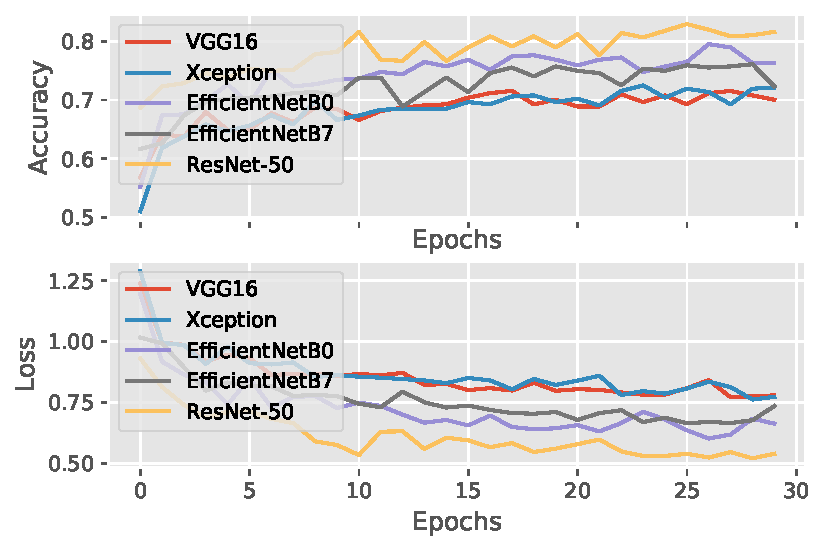
\includegraphics[width=3.1in]{supernet}
\caption{Architectures comparison.}
\label{fig:supernet-comparison}
\end{figure}

According to the results in Figure \ref{fig:supernet-comparison}, the best model was ResNet-50. However, we decided to keep also VGG16 given its fast inference time.

\begin{center}
\begin{tabular}{ l c }
\hline\hline
Xception & 68.31\% \\
EfficientnetB0 & 77.23\% \\
EfficientnetB7 & 73.24\% \\
ResNet-50 & \textbf{79.51}\% \\
VGG16 & 68.69\% \\
\hline\hline
\end{tabular}
\end{center}

\subsection{Classifier}

\subsubsection{Global Average Pooling Layer}

After the convolutional base we initially had a \verb|Flatten| layer, which we later switched to \verb|GlobalAveragePooling2D| to better summarize the output of the feature extractor. The improvements weren't significant, yet there was a reduction in the number of parameters and in training time.

\subsubsection{Dense Layer and Activation}

To decide the number of \verb|Dense| layers, the number of neurons and the type of activation we considered different options with the following rule: \verb|tanh| should be used when the number of layers isn't too much to avoid the vanishing gradient problem, while when more layers were used it was better to use \verb|ReLU|.

Moreover we used the Keras tuner with the HyperBand algorithm\footcite{hyperband} to tune these hyperparameters.

This testing was performed before fine-tuning (section \ref{sec:tuning}).

\begin{center}
\begin{tabular}{ l c }
\hline\hline
VGG16\\
\hline
ReLU, 512 & 73.81\% \\
ReLU, 256 + 128 (x2) + 64 (x2) & 67.36\% \\
tanh, 512 & 69.45\% \\
tanh, 512 + 256 & 69.45\% \\
ReLU, 384 + 256 (Keras tuner) & \textbf{74.95\%} \\
\hline\hline
ResNet-50\\
\hline
ReLU, 384 (Keras tuner) & \textbf{85.39\%}\\
ReLU, 512 & \textbf{85.39\%}\\
\hline\hline
\end{tabular}
\end{center}

For VGG16 we opted for the tuner configuration.

For ResNet-50, the two configurations performed identically, but we ended up choosing 512 neurons because after fine-tuning the performance was better.

\subsubsection{Batch Normalization Layer}

We employed the \verb|BatchNormalization| layer in order to improve gradient propagation and reduce internal covariance.

\subsubsection{Dropout Layer}

\verb|Dropout| was always used after the \verb|Dense| layer for regularization, since on average we saw an increase of 0.76\% in accuracy.

\section{Training techniques}

\subsection{Fine-tuning}\label{sec:tuning}
Initially, transfer learning was performed first by training the classifier with the convolutional base frozen, and then tuning with a lower learning rate with the last layers of the feature extractor unfrozen.

However, the performance wasn't really satisfying, so we decided to introduce the idea of \textbf{multiple passes}.

We thought that the latent representation of the last frozen layers of the feature extractor wasn't still in line with our dataset, so progressively we unfroze more layers and did more fine-tuning with an even lower learning rate.
This gave a great improvement on our validation set as shown in the comparison:

\begin{center}
\begin{tabular}{lcc}
\hline\hline
& VGG16 & (\textit{ResNet-50}) \\
\hline
No fine-tuning & 74.95\% & 85.39\% \\
Unfreeze last 4 (\emph{32}) & 90.13\% & 89.56\% \\
Unfreeze last 8 (\textit{64}) & 91.65\% & \textbf{91.27\%} \\
Unfreeze last 12 (\textit{96}) & \textbf{92.60\%} & 90.32\% \\
\hline\hline
\end{tabular}
\end{center}

\noindent We chose the best fine-tuning configuration for each of the supernets.

\subsection{Class imbalance}\label{sec:cl_imb}

Classes 1 and 6 were severely under-represented, about half the size of the other classes.
So we decided to compute the class weights according to the number of samples: this led to a \textbf{weighted loss function} that gave more weight to the less represented classes when performing backpropagation. As expected, the F1--scores for such classes saw an improvement of about 0.10.

%Strangely enough, the performance only improved when specifying class weights during the first transfer learning pass, while it got worse if we specified it also in fine-tuning.

\section{Model choice}\label{sec:model-choice}

To choose the final model we considered the one built with VGG16, the one with ResNet-50, and a third one: the \textbf{ensemble} of the two by taking the simple average. We compared not only accuracy, but also the F1--scores.

\begin{center}
\begin{tabular}{cc|ccc}
\hline\hline
& & VGG16 & ResNet-50 & Ensemble \\
\hline
\multirow{8}{*}{\rotatebox[origin=c]{90}{ F1--scores }}
& 1 & 0.735 & 0.723 & \textbf{0.739} \\
& 2 & \textbf{0.955} & 0.926 & \textbf{0.955} \\
& 3 & 0.911 & 0.913 & \textbf{0.928} \\
& 4 & \textbf{0.921} & 0.906 & 0.899 \\
& 5 & 0.931 & 0.904 & \textbf{0.933} \\
& 6 & 0.900 & 0.862 & \textbf{0.918} \\
& 7 & \textbf{0.982} & 0.975 & \textbf{0.982} \\
& 8 & \textbf{0.911} & 0.876 & 0.903 \\
\hline
& Acc. & 92.60\% & 91.27\% & \textbf{92.98\%} \\
\hline\hline
\end{tabular}
\end{center}

The ensemble showed an improvement in almost all the metrics, therefore that is the model we chose.

\section{Conclusion}

\subsection{Performance}

Finally, we added TTA (section \ref{sec:tta}) and the results of the final ensemble both on the train, the validation and the remote test set are as follows:

\begin{center}
\begin{tabular}{ l c c }
\hline\hline
           & Without TTA & With TTA \\
\hline
Train acc. & 99.30\%     & \textbf{99.80}\% \\
Val acc.   & 92.98\%     & \textbf{94.50}\% \\
Test acc.  & 89.16\%     & \textbf{91.40}\% \\
\hline\hline
\end{tabular}

\end{center}

\noindent The final confusion matrix can be seen in Figure \ref{fig:confusion}.

\begin{figure}[h!]
\centering
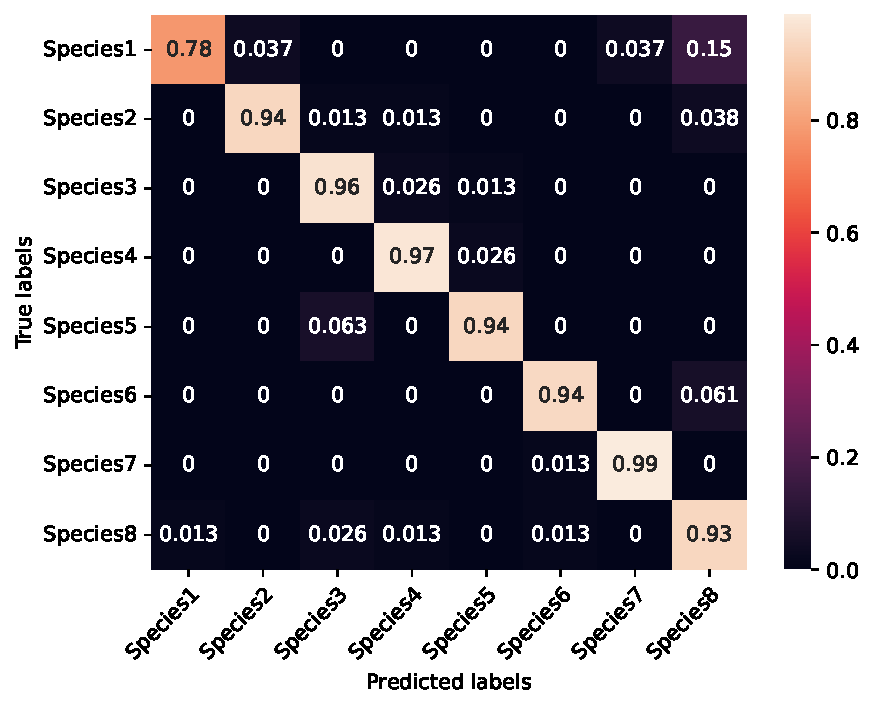
\includegraphics[width=3.3in]{confusion}
\caption{Confusion matrix on the validation set of the final model.}
\label{fig:confusion}
\end{figure}

\subsection{Further Developments}

We acknowledge that our workflow might use some additional procedure, for example an exploitation of more advanced augmentation techniques, in order to help the generalization power of the model. Moreover, we could experiment with more advanced pretrained models, different optimizers and learning rates.

It can be seen that, although we introduced class weights (section \ref{sec:cl_imb}) to tackle class imbalance, the F1-scores of the underrepresented classes are still lower than the ones of the other classes: further procedures may be implemented to handle this issue.

Taking account of these considerations, and given the limited resources at our disposal, we are satisfied with the results.

\end{document}